\documentclass[pdftex,12pt,a4paper]{article}
\usepackage[pdftex]{graphicx}
\usepackage{xcolor}
\usepackage{marginnote}
\usepackage{enumitem}
\usepackage{multirow}
\usepackage{subcaption}
\usepackage{titlesec}
\usepackage[bottom=1.5cm, outer=5cm, inner=2cm, heightrounded,
marginparwidth=4cm, marginparsep=0.5cm]{geometry}
\titleformat{\section}{\bfseries}{\Large Question \thesection: }{0em}{}

\begin{document}
    % Custom title page
    \begin{titlepage}
        \begin{center}
            
\includegraphics[width=5cm]{figures/kulogo}\\[1cm]
            {\large \bfseries
                Spring 2014\\
                Computer Networks\\
                CMPE323\\[1cm]
            }
            {\large \bfseries
                \noindent Quiz 3\\[1cm]
            }
        \end{center}

        \begin{center}
            \begin{tabular}{|c|p{1cm}l|}\hline
                \textbf{Questions} & \multicolumn{2}{|c|}{\textbf{Points}} \\\hline
                Q1                &    &    /$\frac{100}{3}$\%   \\\hline
                Q2                &    &    /$\frac{100}{3}$\%   \\\hline
                Q3                &    &    /$\frac{100}{3}$\%   \\\hline
            \end{tabular}
        \end{center}

        \vfill
        \begin{tabular}{lp{5cm}ll}
            \textbf{Student name:} & & \textbf{Student ID:} & \\
        \end{tabular}


    \end{titlepage}
    \newpage

    % quiz content
    \section{}

        \begin{figure}[tbh]
            \centering
            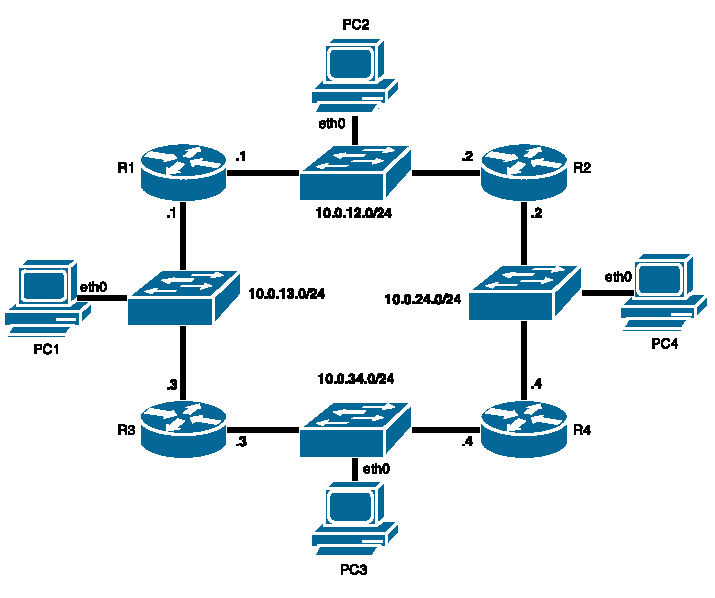
\includegraphics[width=.85\textwidth]{figures/diag0}
            \caption{Four inter-connected networks.}
            \label{fig1}
        \end{figure}

        Consider Figure \ref{fig1} where the routers R1, R2, and R3 are all
        correctly configured with RIPv2 such that any node in the network can
        ping any node.
        
        \textbf{Questions:} if you view the routing table of R3 (i.e. using the command \texttt{show ip
        route}), what would be the answer of the following questions:
        \begin{itemize}
            \item What would be the next-hop IP address (aka via address) for
                reaching the network \texttt{10.0.12.0/24}?
            \item What would be the metric that is associated with the route of
                the same network (i.e. \texttt{10.0.12.0./24})?
            \item From the perspective of R3, what would be the metric of the
                updates that are received from R1 for the same network?
            \item From the perspective of R3, what would be the metric of the
                updates that are received from R4 for the same network?
        \end{itemize}


        \pagebreak

    \section{}
        Given the same topology as depicted in Figure \ref{fig1} and knowing
        that the default gateway of PC1 is R1, what would be the content of the
        Access-Control List (ACL) that, if applied as a firewall rule in R1,
        would result in permitting all packets except dropping ones that
        meet the following criteria:
        \begin{itemize}
            \item From PC1 that go to any PC in the network \texttt{10.0.12.0/24},
            \item AND using the TCP protocol,
            \item AND using the destination port 80,
        \end{itemize}

        Use the following syntax to describe the ACL entries (note: there is an
        implicit deny at the end of the ACL): 
        
        \texttt{<action> <proto> <sip> <wmask> [eq <sp>] <dip> <wmask> [eq
        <dp>]}
        \vspace{0.2cm}

        Where:
        \begin{itemize}
            \item \texttt{<action>} is either \texttt{permit} or \texttt{deny}.
            \item \texttt{<proto>} is either \texttt{ip}, \texttt{tcp}, \texttt{udp}, or \texttt{icmp}.
            \item \texttt{<sip>} is the source IP address.
            \item \texttt{<dip>} is the destination IP address.
            \item \texttt{<wmask>} is a wild-card mask (the opposite of a subnet
                mask, a bit of 0 corresponds to a bit that must match, and 1
                for otherwise).
        \end{itemize}

        \textbf{Questions:}
        \begin{itemize}
            \item Write down the content of the ACL using the syntax above.
            \item What is the interface on R1 that you would apply the ACL on
                (mark a circle on the interface in Figure \ref{fig1})?
            \item What is the direction by which you apply the ACL on the
                interface (i.e.  inbound or outbound to the router)?
        \end{itemize}

        \pagebreak

        \section{}
            Consider the same topology as depicted in Figure \ref{fig1}, and
            assume the following:
            \begin{itemize}
                \item PC2 and PC4 use R2 as their default gateway.
                \item R2 has NAPT (Network Address and Port Translation)
                    configured such that packets that are sourced from
                    10.0.24.0/24 and destined to 10.0.12.0/24 have their source
                    addresses translated.
                \item The address translation aims at allowing maximum number of
                    connections from 10.0.24.0/24 to 10.0.12.0/24 such that the
                    translated source IP address is 10.0.12.2.
                \item PC4 sent a UDP packet to PC2 with the source port of
                    50,000 and the destination port of 53.
            \end{itemize}

            \textbf{Question:}
            \begin{itemize}
                \item What would be a valid NAPT translation entry in the NAT
                    table of R2:
                    \begin{itemize}
                        \item Protocol:
                        \item Source IP address:
                        \item Destination IP address:
                        \item Source port:
                        \item Destination port:
                    \end{itemize}
            \end{itemize}




\end{document}
